Une large partie de la théorie des données fonctionnelles suppose que l'on observe des courbes $X_i : \Omega \rightarrow \mathcal C^0(I, \mathds R)$ \textbf{indépendantes} et identiquement distribuées. Cependant une partie non négligeable des données que l'on observe ont des dépendances avec les valeurs passées. Par exemple, il est raisonnable de penser que la consommation électrique d'un foyer au cours d'une année croît avec l'ajout successif de nouveau appareils électroniques. L'hypothèse d'indépendance entre les données n'est donc plus pertinente pour les données que l'on traite et il devient important de considérer des processus autorégressifs adaptés aux données fonctionnelles.
Si dans le cadre des données de $\mathds R$ cette relation de \emph{dépendance linéaire} avec le passé pouvait s'écrire sous la forme suivante
$X_n = \sum\limits_{k=1}^{n-1} \varphi_k \, X_k + \xi_n$ où $\varphi_k \in \grandR$
et
$\xi_n \begin{cases} \in \operatorname{VA}(\grandR) \\ \indep \sigma\left( X_i \right)_{1\,: \, n-1}\end{cases}$,
dans le cadre fonctionnel on capture la même idée en considérant
$X_n = \sum\limits_{k=1}^{n-1} \phi_k \left( X_k \right) + \xi_n$ où $\phi_k$
est un \emph{opérateur linéaire} de $\mathds L^2(I, \mathds R)$,
le plus souvent intégral.

\chk{
    Il s'agit d'une généralisation naturelle de la relation dans le cadre réel, puisqu'on peut démontrer que sur l'espace des nombres réels l'ensemble des fonctions linéaires $\phi : \grandR \rightarrow \grandR$ sont de la forme $x \mapsto ax$ avec $a \in \grandR$. La relation sur $\grandR$ que l'on a vue juste avant peut alors se ré-écrire de façon similaire à la version fonctionnelle.
}

On considère lors de ce stage des séries temporelles de données fonctionnelles car les données que l'on manipule ( en l'occurence les données de courbe de charge des parcs éoliens ) semblent être naturellement corrélées dans le temps.


\question{Pourquoi se soucier en particulier des séries temporelles fonctionnelles lorsque l'on souhaite incorporer la régularité du processus dont est issu nos données dans l'estimation des quantités qui nous intéressent ?}

Rappelons-nous que les données fonctionnelles sont la clé pour déterminer la régularité, et que cela est en réalité permis par le théorème de \nameref{rem:kolmo_continuite} (que nous n'avons pas énoncé en détails, mais mentionné dans la section \ref{sec:informel}). Malheureusement, dans le monde réel où vit le praticien, nous n'avons pas accès à l'espérance de la loi dont sont issues nos données. Il nous faut donc estimer cette espérance, et c'est là que les séries temporelles fonctionnelles entrent en jeu. Puisque l'estimateur usuel de l'espérance est la moyenne empirique, qui nous est fourni par la loi des grands nombres, cela devient très problématiques lorsque l'on dispose de données corrélées. Ce que nous allons voir, c'est que l'on peut tout de même utiliser l'estimateur usuel de l'espérance, et que l'on obtiendra des estimateurs des paramètres de régularité convergents ponctuellement vers ceux du processus dont sont issues nos données. Ce résultat, dû à MPV, nécessitera toutefois de faire d'abord un détour sur ce qu'on entend par dépendance.

\begin{figure}[H]
    \centering
    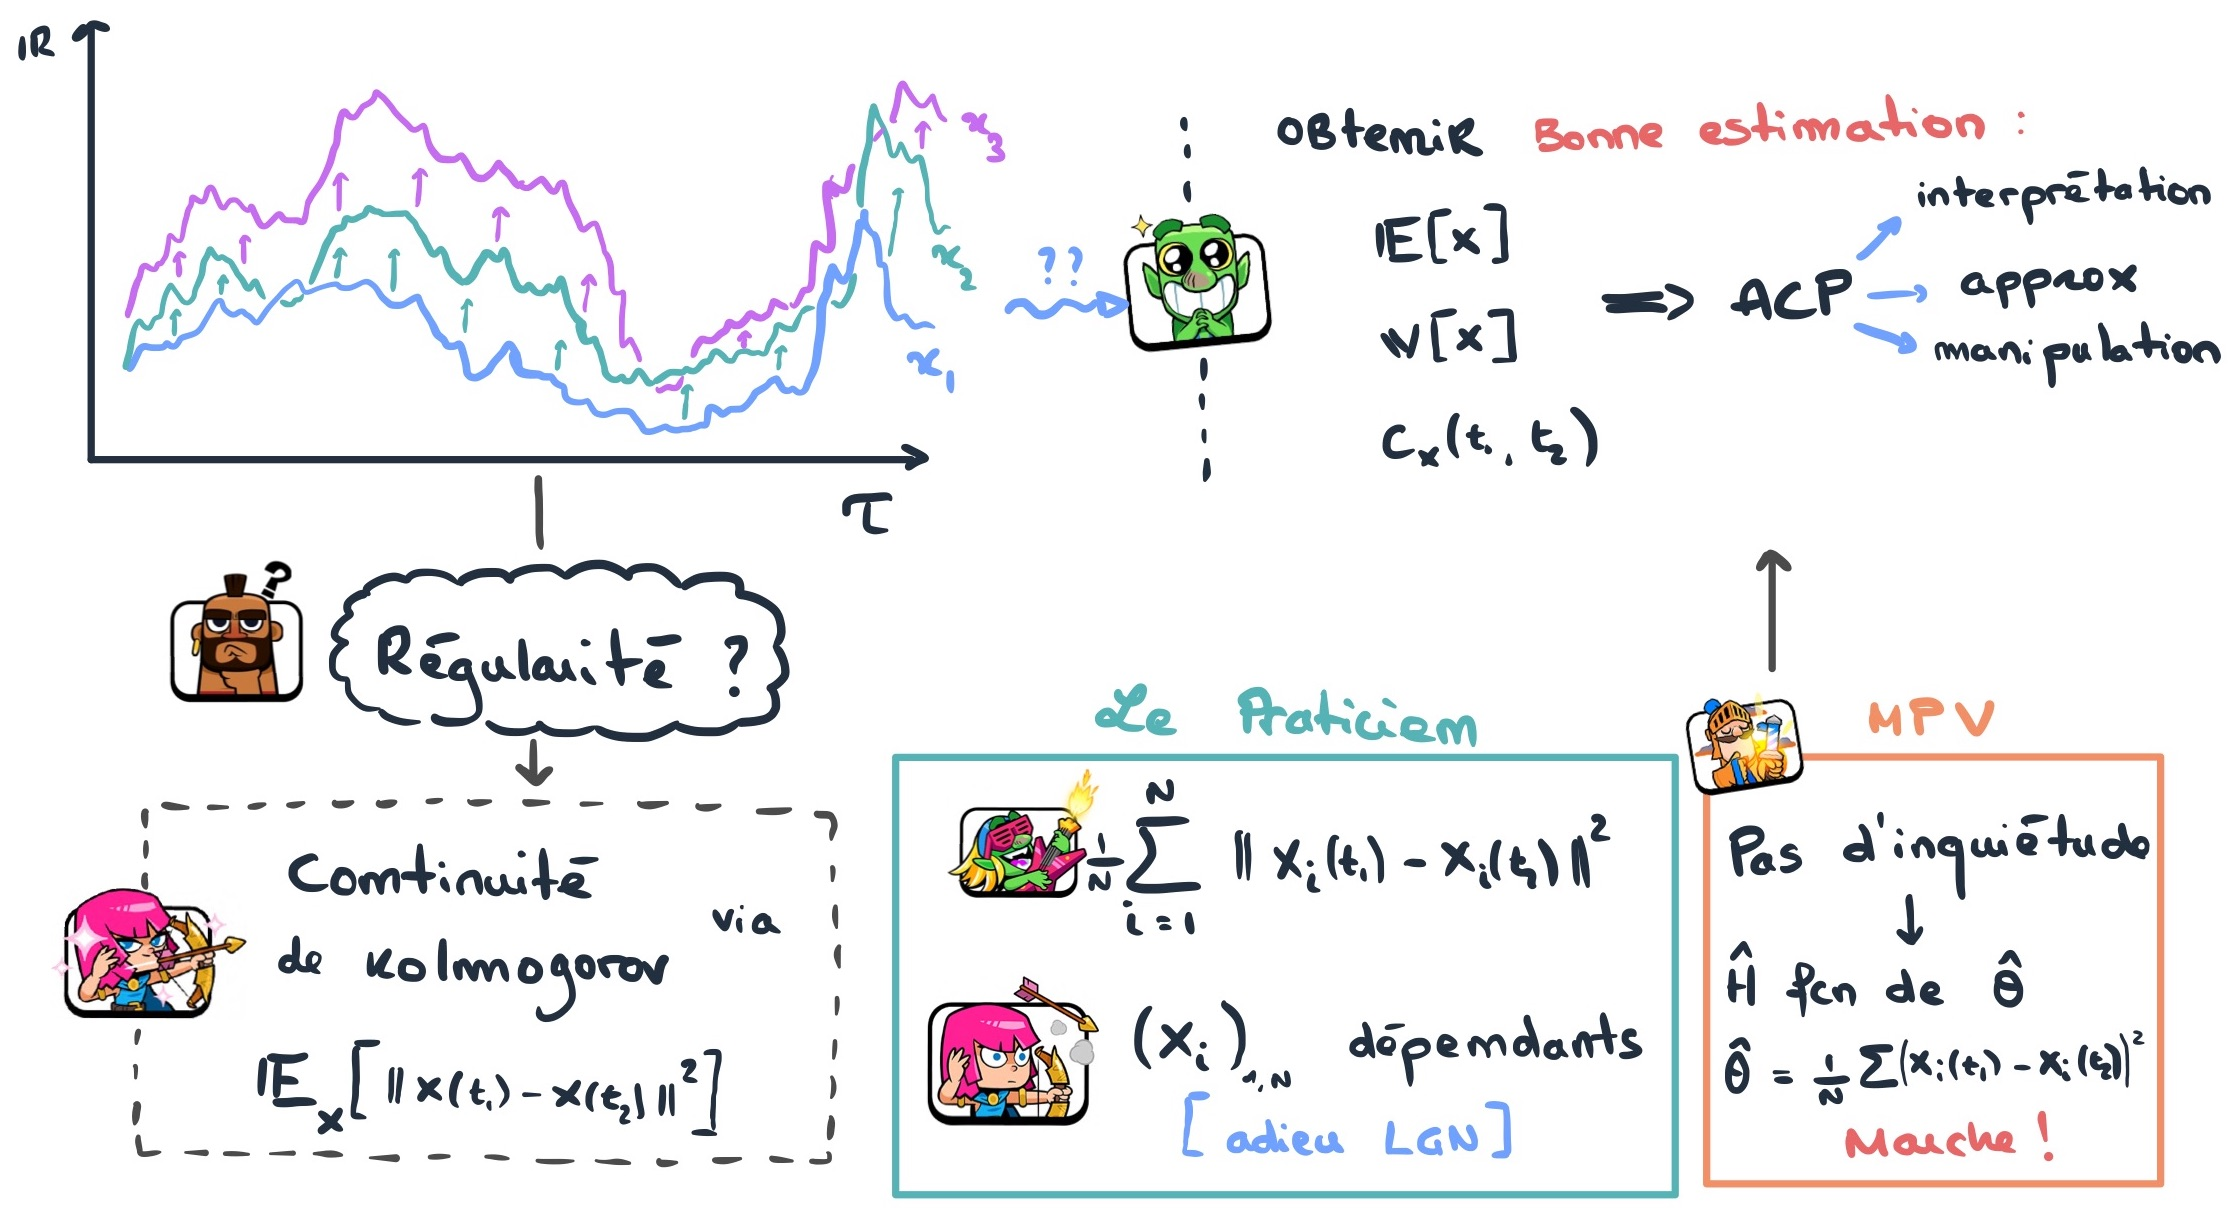
\includegraphics[width=\textwidth]{Images/sketches/schema_ts_estim_reg.jpg}
    \caption{Schéma grossièrement récapitulatif : Estimation de la régularité pour une série temporelle fonctionnelle}
    \label{fig:recap_estim_reg_fts}
\end{figure}
